\chapter{Theoretical Background}
\label{ch:theo-back}

For a proper understanding of this documentation and the ideas explained on it, it is
needed to know some theoretical concepts that are the fundaments of Linked Data, RDF,
RDF Validation, programming languages and compilers. For
those readers that want a more detailed view of the concepts
presented here is offered in \cite{labra-validating-rdf, eric-rdf-validation-lang,
programing-language}.

% S E C T I O N   R D F

\section{RDF}
\label{sec:theo-back-rdf}
Resource Description Framework (RDF) is a standard model for data interchange on the web.
It started in 1998 and the first version of the specification was published in 2004 by the W3C
according to \cite{rdf-primer}. RDF has features that facilitate data merging even if the
underlying schemas differ, and it specifically supports the evolution of schemas over time
without requiring all the data consumers to be changed. Another important feature is that RDF
supports XML, N-Triples and Turtle syntax. The most common representation though is the N-Triples syntax.
It it composed of a set of triples. Each triple is composed of three elements, the subject the predicate and the
object. The \cref{fig:rdf-ntriples-ex} shows an example of how a triplet can be written in RDF N-Triples Syntax.

\begin{figure}
\begin{lstlisting}[numbers=left, basicstyle=\ttfamily\scriptsize]
<http://example/subject1> <http://example/predicate1> <http://example/object1> .
\end{lstlisting}
\caption[RDF N-Triples Example]{RDF N-Triples Example. From this example we can see that each triplet is
composed of three elements, the subject the predicate and the object.}
\label{fig:rdf-ntriples-ex}
\end{figure}

RDF extends the linking structure of the Web to use URIs to name the relationship between
things as well as the two ends of the link, this is usually referred to as a “triple” or "triplet".
As we can see from \cref{fig:rdf-ntriples-ex} each triple it is composed of three elements,
the subject, the predicate and the object. Each one of them can contain any URI value.
Using this simple model, it allows structured and semi-structured data to be mixed, exposed,
and shared across different applications. \cref{fig:rdf-graph} shows an example of how different
triples can be use to compose a graph, this graph represents the same as the \cref{fig:rdf-ntriples-graph}

\begin{figure}
\begin{lstlisting}[numbers=left, basicstyle=\ttfamily\scriptsize]
<http://example/bob> <http://example/knows> <http://example/alice> .
<http://example/alice> <http://example/knows> <http://example/peter> .
\end{lstlisting}
\caption[RDF N-Triples Graph Example]{RDF N-Triples Graph Example. This example shows the n-triples
that generate the graph from \cref{fig:rdf-graph}.}
\label{fig:rdf-ntriples-graph}
\end{figure}

This linking structure forms a directed, labelled graph, where the edges represent the named link
between two resources, represented by the graph nodes. This graph view is usually used for an easy understanding of the RDF model.

Also, related to this we strongly recommend the Tim Berners-Lee’s writings on Web Design Issues
\cite{semantic-roadmap} where he explain the issues of the liked data and why is RDF so important.

\begin{figure}
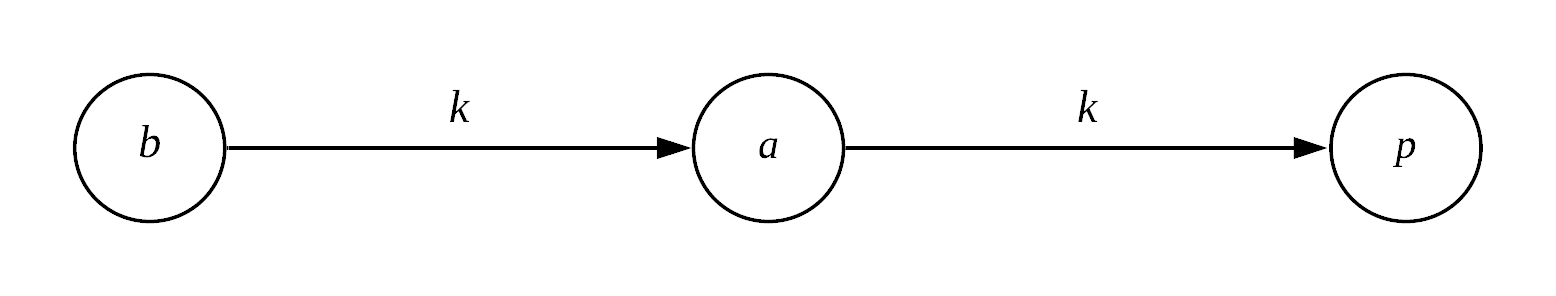
\includegraphics[scale=0.2]{images/shex-lite-rdf-graph.png}
\centering
\caption[RDF Example graph]{RDF graph formed by triplets from \cref{fig:rdf-ntriples-graph}, where
\textit{b} corresponds to \textit{\texttt{<http://example/bob>}}, \textit{a} corresponds to
\textit{\texttt{<http://example/alice>}}, \textit{p} corresponds to \textit{\texttt{<http://example/peter>}}
and \textit{k} corresponds to \textit{\texttt{<http://example/knows>}}.}
\label{fig:rdf-graph}
\end{figure}

% S E C T I O N   V A L I D A T I N G   R D F

\section{Validating RDF}
RDF therefore allows to represent and store data, and with this ability emerges the need to validate
that the schema of the graph is correct. In order to perform the validation of RDF data there have
been previous attempts, described in \cref{sec:theo-back-rdf}, this dissertation will focus
on Shape Expressions. But, in order to validate RDF data, every technology needs to face the following
RDF concepts:

\begin{itemize}
 \item The form of a node (the mechanisms for doing this will be called “node constraints”).
 \item The number of possible arcs incoming/outgoing from a node.
 \item The possible values associated with those arcs.
\end{itemize}

\begin{figure}
  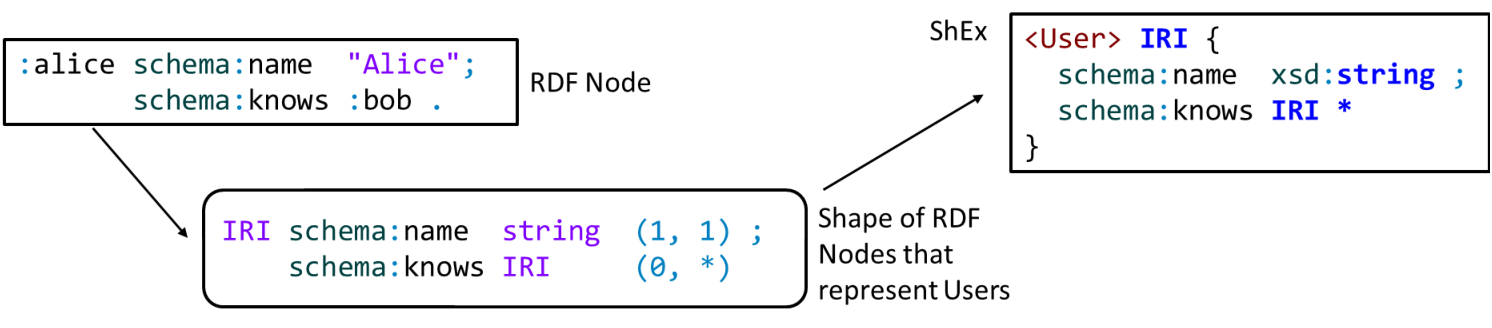
\includegraphics[scale=0.25]{images/rdf-node-and-shape.png}
  \centering
  \caption[RDF node and its shape]{RDF node and its shape.}
  \label{fig:rdf-graph-2}
\end{figure}

\cref{fig:rdf-graph} illustrates those RDF concepts by means of the Shape Expression that validates users.
There we can see that the shape of the RDF node that represents Users represents the form of a node,
the number of possible arcs and the possible value associated with those arcs.

\subsection{Shape Expressions}
As defined in \cite{labra-validating-rdf}, Shape Expressions (ShEx) is a schema language for describing RDF
graphs structures. ShEx was originally developed in late 2013 to provide a human-readable syntax for OSLC
Resource Shapes. It added disjunctions, so it was more expressive than Resource Shapes. Tokens in the language
were adopted from Turtle and SPARQL with tokens for grouping, repetition and wildcards from regular expression
and RelaxNG Compact Syntax \cite{van2003relax}. The language was described in a paper
\cite{eric-rdf-validation-lang} and codified in a June 2014 W3C member submission, which included a primer and
a semantics specification. This was later deemed “ShEx 1.0”.

As of publication, the ShEx Community Group was starting to work on ShEx 2.1 to add features like value comparison
and unique keys. See the ShEx Homepage \url{http://shex.io/} for the state of the art in ShEx. A collection of
ShEx schemas has also been started at \url{https://github.com/shexSpec/schemas}.

\begin{figure}
\begin{lstlisting}[numbers=left, basicstyle=\ttfamily\scriptsize]
PREFIX :       <http://example.org/>
PREFIX schema: <http://schema.org/>
PREFIX xsd:  <http://www.w3.org/2001/XMLSchema#>

:User {
  schema:name          xsd:string  ;
  schema:birthDate     xsd:date?  ;
  schema:gender        [ schema:Male schema:Female ] OR xsd:string ;
  schema:knows         IRI @:User*
}
\end{lstlisting}
\caption[Shape Expression Example]{Shape Expression Example. This example describes a shape expression that
models a user as a node that has one name of type string, an optional birth date of type date, one gender
of type Male, Female or free string and a set between 0 and infinite of other users represented by the knows
property.}
\label{fig:shape-expr-ex}
\end{figure}

\subsubsection{ShEx Compact Syntax: \texttt{ShExC}}
The ShEx compact syntax (ShExC) was designed to be read and edited by humans. It follows some conventions which
are similar to Turtle or SPARQL.

\begin{itemize}
    \item \texttt{PREFIX} and \texttt{BASE} declarations follow the same convention as in Turtle. In the rest of
    this chapter we will omit prefix declarations for brevity.
	\item Comments start with a \texttt{\#} and continue until the end of line.
	\item The keyword a identifies the \texttt{rdf:type} property.
    \item Relative and absolute IRIs are enclosed by \texttt{< >} and prefixed names (a shorter way to write
    out IRIs) are written with prefix followed by a colon.
	\item Blank nodes are identified using \texttt{\_:label} notation.
    \item Literals can be enclosed by the same quotation conventions ( \texttt{'}, \texttt{"}, \texttt{'''},
    \texttt{"""}) as in Turtle.
    \item Keywords (apart from a) are not case sensitive. Which means that \texttt{MinInclusive} is the same
    as \texttt{MININCLUSIVE}.
\end{itemize}

A ShExC document declares a ShEx schema. A ShEx schema is a set of labelled shape expressions which are composed
of node constraints and shapes. These constrain the permissible values or graph structure around a node in an RDF
graph. When we are considering a specific node, we call that node the focus node.

\begin{figure}
  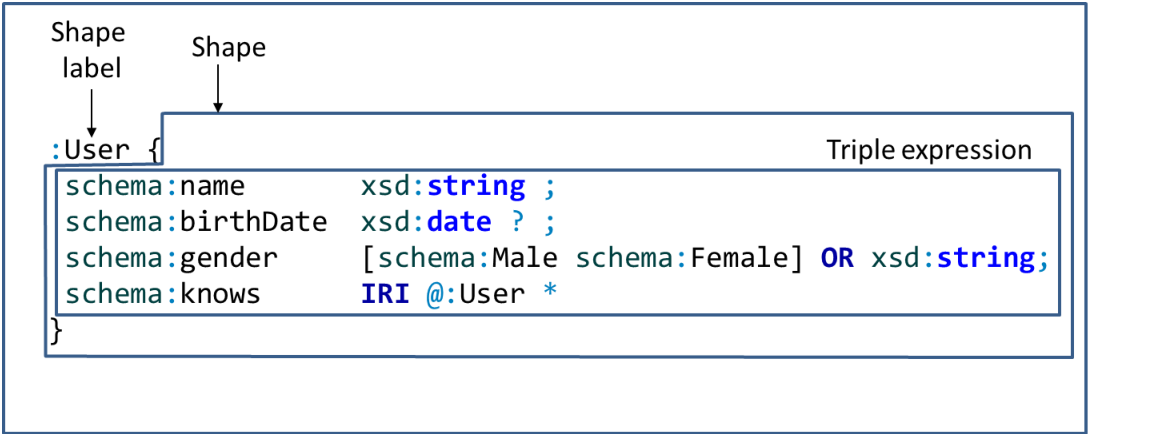
\includegraphics[scale=0.25]{images/shex-out.png}
  \centering
  \caption[Shapes, shape expression labels and triple expressions]{Shapes, shape expression labels and triple expressions.}
  \label{fig:shex-out-view}
\end{figure}

\cref{fig:shex-out-view} shows the first level of a shape expression, we have a label and the shape itself that is
what we assign to the \texttt{:User} label. Then, the shape is composed by triple expressions. The triple expression
structure is explained in \cref{fig:shex-triple-expression}, and as its name indicates it is composed of three
elements, the property, the node constraint and the cardinality.

\begin{figure}
  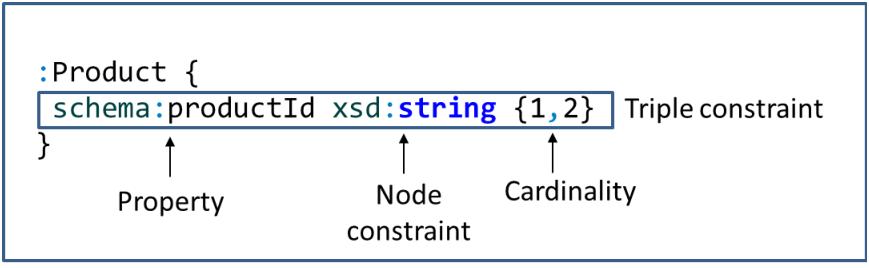
\includegraphics[scale=0.25]{images/shex-triple-expression.png}
  \centering
  \caption[Parts of a triple expression]{Parts of a triple expression.}
  \label{fig:shex-triple-expression}
\end{figure}

Shape Expressions Compact Syntax is much bigger and contains other multiple features that give ShEx its power,
and all of them can be explored in \cite{labra-validating-rdf} but they are not needed to understand this
dissertation.

\subsubsection{Use of ShEx}
Strictly speaking, a ShEx schema defines a set of graphs. This can be used for many purposes, including
communicating data structures associated with some process or interface, generating or validating data,
or driving user interface generation and navigation. At the core of all of these use cases we have the notion
of conformance with schema. Even when someone is using ShEx to create shapes, the goal is to accept and present
data which is valid with respect to a schema. ShEx has several serialization formats:

\begin{itemize}
	\item a concise, human-readable compact syntax (ShExC);
	\item a JSON-LD syntax (ShExJ) which serves as an abstract syntax; and
	\item an RDF representation (ShExR) derived from the JSON-LD syntax.
\end{itemize}

These are all isomorphic and most implementations can map from one to another.
Tools that derive schemas by inspection or translate them from other schema languages typically generate ShExJ.
Interactions with users, e.g., in specifications are almost always in the compact syntax ShExC. As a practical
example, in HL7 FHIR\footnote{\url{https://www.hl7.org/fhir/}}, ShExJ schemas are automatically generated from other formats, and presented to the end
user using compact syntax.

ShExR allows to use RDF tools to manage schemas, e.g., running a SPARQL query to find out whether an organization
is using \texttt{dc:creator} with a \texttt{string}, a \texttt{foaf:Person}, or even whether an organization is consistent about it.

\subsubsection{ShEx Implementations}
At the time of this writing, we are aware of the following implementations of ShEx.

\begin{itemize}
	\item shex.js for Javascript/N3.js (Eric Prud’hommeaux) \url{https://github.com/shexSpec/shex.js/};
	\item Shaclex for Scala/Jena (Jose Emilio Labra Gayo) \url{https://github.com/labra/shaclex/};
	\item shex.rb for Ruby/RDF.rb (Gregg Kellogg) \url{https://github.com/ruby-rdf/shex};
	\item Java ShEx for Java/Jena (Iovka Boneva/University of Lille) \url{https://gforge.inria.fr/projects/shex-impl/}; and
	\item ShExkell for Haskell (Sergio Iván Franco and Weso Research Group) \url{https://github.com/weso/shexkell}.
\end{itemize}

There are also several online demos and tools that can be used to experiment with ShEx.

\begin{itemize}
	\item shex.js (http://rawgit.com/shexSpec/shex.js/master/doc/shex-simple.html);
	\item Shaclex (http://shaclex.herokuapp.com); and
	\item ShExValidata (for ShEx 1.0) (https://www.w3.org/2015/03/ShExValidata/).
\end{itemize}

\subsection{Other Technologies}
\label{subs:theo-back-validating-other-techs}
As other validation technologies it is very interesting to know how
other tools approach the same issue.

\subsubsection{SHACL}
From \cite{labra-validating-rdf}, Shapes Constraint Language (SHACL)
has been developed by the W3C RDF Data Shapes Working Group, which was chartered in 2014 with the goal to “produce
a language for defining structural constraints on RDF graphs \cite{oslc-resource-shape}.”

The main difference that made us choose ShEx over SHACL is that ShEx emphasized human readability, with a
compact grammar that follows traditional language design principles and a compact syntax evolved from Turtle.

\subsubsection{JSON Schema}
JSON Schema born as a way to validate JSON-LD, and as turtle and RDF can be serialized as JSON-LD, it is usual to
think that JSON Schema can validate RDF data, but this is not fully correct. And the reason is that the serialization
of RDF data in to JSON-LD is not deterministic, that means that a single schema might have multiple serializations,
which interferes with the validation as you cannot define a relative schema.

% S E C T I O N   P R O G R A M M I N G   L A N G U A G E S

\section{Programming Languages}
According to \cite{programing-language}, \textit{“a programming language is a formal language comprising a set of instructions
that produce various kinds of output.”} When we talk about programming languages we need to know that they are split into
two categories, General Purpose Languages (GPL) and Domain Specific Languages (DSL). The main difference overtime is that, as stated
in \cite{dsl}, a domain-specific language (DSL) is a computer language specialized to a particular application domain
in contrast to a general-purpose language (GPL), which is broadly applicable across domains.

In the specific case of ShEx-Lite, we will be talking about a Domain Specific Language, and, more specifically, a declarative one, we would classified
it as a Declarative one, that means that it is not Touring Complete \cite{touring-complete}.

% S E C T I O N   C O M P I L E R S

\section{Compilers}
A compiler is a computer program that translates computer code written in one programming language (the source language)
into another language (the target language). Is during this translation process where the compiler validates the syntax
and the semantics of the program, if any error is detected in the process the compiler raises an exception (understand
as a compiler event that avoids the compiler to continue its execution).

\subsection{Internal Structure}
In order to decompose the internal structure of a compiler, they have been split into the most common task they do
(\cref{fig:compiler-stages}). This does not mean that there are compilers that might have more or less stages. But at the
end, everything can be grouped into any of the stages that we will explain:

\begin{figure}
  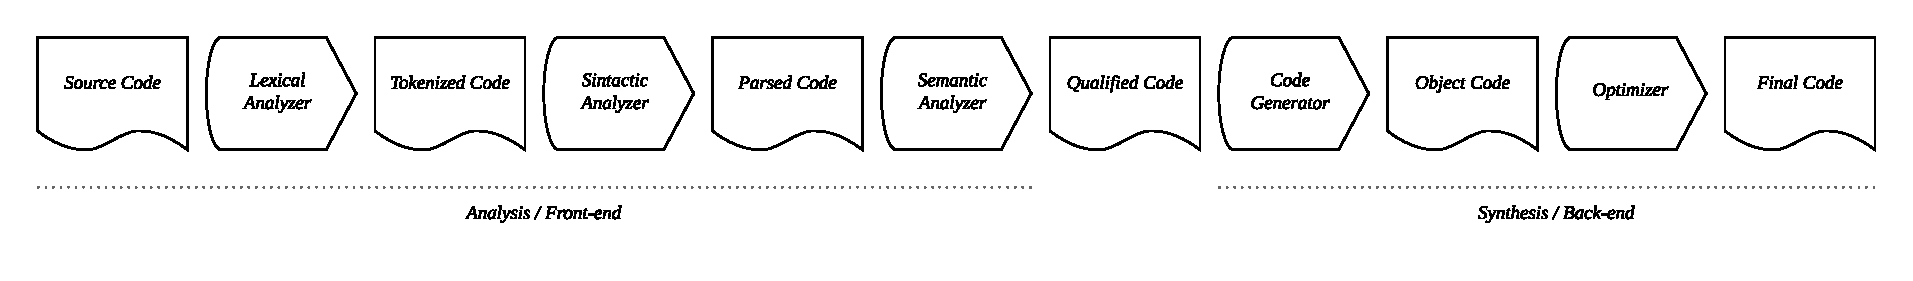
\includegraphics[width=\textwidth]{images/compiler-stages.pdf}
  \centering
  \caption[Compiler stages]{Compiler stages.}
  \label{fig:compiler-stages}
\end{figure}

\subsubsection{Lexical Analyser}
The lexical analyser task is to get the input and split it in to tokens \cite{lexical-analysis}, which are build
from lexemes. If the compiler cannot find a valid token for some lexemes in the source code, it will generate an error,
as the input cannot be recognized.

\subsubsection{Syntactic Analyser}
The syntactic analyser takes the tokens generated during the lexical analysis and try’s
to group the tokens so the conform to the language grammar rules. During this stage, if there is any error while trying to
group the tokens, then the compiler will rise an error as the input cannot be parsed.

\subsubsection{Semantic Analyser}
The semantic analyser has two main tasks, usually. First, it validates that the source code semantics are correct. For
example in java 4 + “aaa” would not make sense as the semantic rules specify that and integer cannot be added to an string.
And the second task is to transform the Abstract Syntax Tree in to a type-checked
and annotated AST. Usually that means relate the invocations and variables to its definition, very useful for type-checking.

\subsubsection{Code Generator}
The task of the code generator as its name indicates is to generate the target code. It can be byte code, machine code,
or even another high-language code.

\subsubsection{Code Optimizer}
The code optimizer is the last step before the final target code is generated, it rewrites the code that the code generator
produced without changing the semantics of the program, its aim is just to make code faster. At \cite{compiler-optimizations}
you can see an example of some optimizations that can be done at compile time to make your code faster.

\subsection{Conventional Compilers}
Conventional compilers are a big monolith where each stage \ref{fig:compiler-stages} is executed automatically after the
previous stage, if the compiler has eight steps you need to execute them all at once. This approach presents some drawbacks:
\begin{itemize}
    \item A poor IDE \cite{ide} integration. IDE’s need to perform incremental compilations in matter of nanoseconds so
    the user doesn’t feel lag when typing the program. With conventional compilers as you need to go through all the compilation
    process at once they where very slow and companies like Microsoft need to develop different compilers, one for the IDE and
    another for the final compilation of the program itself. This lead to several problems like that if a feature gets
    implemented in the final compilation compiler but not in the IDE one the IDE would not support the feature meanwhile
    the language would.
    \item Difficult to debug. As the conventional compilers where a black box the only way to test intermediate stages was
    by throwing an input and waiting the the feature you wanted to test was thrown for that input.
\end{itemize}

\subsection{Modern Compilers}
After the problems Microsoft had with the C\# compiler they decide to rewrite the whole compiler and introduce a concept
called “compiler as an API” with Roslyn \cite{dotNet}. This concept has been perfectly accepted and solved many problems,
such as incremental compilation.
In this concept each stage has an input and an output that can be accessed from outside the compiler, and stages can be
executed independently on demand. For example if an IDE just want to execute the Lexer the Parser and
the Semantic analysis it can. That translates in to speed for the user.

Also the second problem is solved as testing individual parts of the compiler is much more easy than the hole compiler
at once.
